\documentclass[conference]{IEEEtran}
\IEEEoverridecommandlockouts
\usepackage{cite}
\usepackage{amsmath,amssymb,amsfonts}
\usepackage{graphicx}
\graphicspath{{../diagrams/}{docs/diagrams/}}
\usepackage{textcomp}
\usepackage{xcolor}
\usepackage{booktabs}
\usepackage{url}
\usepackage{listings}

\begin{document}

\title{Design, RTL Implementation, and Empirical Evaluation of a Level-1 Split-Cache Memory Hierarchy in Modified Harvard Architecture\thanks{Demonstration Video: \url{https://drive.google.com/file/d/1w4z_5gOMVCfHtYa4Goujhmb_GkWyMnq4/view?usp=sharing}. GitHub Repository: \url{https://github.com/vs-code06/MCA_Project.git}}\\
{\footnotesize \textsuperscript{*}Course: Modern Computer Architecture (MCA) --- Project 9 (Phase II Final Report)}}

\author{
\IEEEauthorblockN{\textbf{Team: Decoders07}}
\IEEEauthorblockN{Anant Jain (2401010066), Vipul Sharma (2401010505), Krishna Gehlot (2401010236),}
\IEEEauthorblockN{Aditya Kumar (2401010029), and Kartik Mehra (2401020030)}
\IEEEauthorblockA{\textit{Department of Computer Science and Engineering, Newton School of Technology} \\
\textit{Rishihood University, Sonipat, India}}
}

\maketitle

\begin{abstract}
While pure Harvard architectures physically isolate instruction and data paths to eliminate structural hazards, practical high-performance microprocessors face physical memory limits and access latencies when scaling to multi-megabyte or gigabyte address spaces. To bridge this processor-memory speed disparity while preserving concurrent dual-port bandwidth at the core boundary, modern systems adopt a \textit{Modified Harvard Architecture}. In this paradigm, dedicated Level-1 Instruction (L1 I-Cache) and Level-1 Data (L1 D-Cache) caches sit directly adjacent to the processor pipelines, backed by a unified, multi-cycle shared main memory subsystem. 

In this Phase~II work, Team \textbf{Decoders07} designs, implements in synthesizable Verilog HDL, and empirically verifies a complete Level-1 cache hierarchy with backing multi-cycle main memory. The system incorporates: (1) a 16-line direct-mapped L1 I-Cache with single-cycle hit output and line refill finite state machine (FSM); (2) a 16-line direct-mapped L1 D-Cache featuring a Write-Through policy, No-Write-Allocate on write misses, and 4-byte lane masking; (3) a multi-cycle shared main memory subsystem (1024 words, 4~KB) with a priority bus arbiter ($D > I$) and configurable memory wait-state latency; and (4) real-time hardware telemetry counters computing Average Memory Access Time (AMAT) and hit/miss rates. Cycle-accurate behavioral simulations using Icarus Verilog demonstrate that on iterative loop workloads, the L1 caches achieve an $82.76\%$ instruction hit rate ($\text{AMAT}_I = 1.52$ cycles) and a $72.73\%$ data hit rate ($\text{AMAT}_D = 1.82$ cycles), successfully shielding the core from 3-cycle memory wait states. A 3-way comparative benchmark systematically contrasts Pure Harvard (Phase 1), Shared-Memory Von Neumann (Phase 1), and Modified Harvard with Caches (Phase 2).
\end{abstract}

\begin{IEEEkeywords}
Modified Harvard Architecture, Level-1 Cache, Direct-Mapped Cache, Write-Through, Average Memory Access Time (AMAT), Bus Arbitration, Memory Hierarchy, Verilog HDL.
\end{IEEEkeywords}

\section{Introduction}
As microprocessor operating frequencies have scaled by orders of magnitude over recent decades, off-chip dynamic RAM (DRAM) access latencies have improved at a significantly slower pace, creating the classic ``Memory Wall'' \cite{wulf1995hitting}. To maximize instruction throughput, processors cannot afford to incur full main memory latency on every instruction fetch and memory operand reference.

In Phase~I, our team demonstrated that a pure Harvard architecture eliminates structural bus conflicts by providing completely segregated physical memories and buses for code and data, achieving an ideal Cycles Per Instruction ($\text{CPI} = 1.00$) and a $1.47\times$ speedup over a unified Von Neumann baseline \cite{hennessy2019computer}. However, a pure Harvard model with ideal single-cycle memories at infinite capacity is physically and economically unfeasible in general-purpose computing. Large storage arrays inevitably suffer from capacitive wire delays, multi-cycle propagation times, and pin-count constraints.

To resolve these physical constraints, industry-standard microprocessors (including ARM Cortex-A and Intel x86 architectures) deploy a \textbf{Modified Harvard Architecture} \cite{patterson2020computer, shen2013modern}. In this hierarchy:
\begin{itemize}
    \item \textbf{Level-1 Core Boundary:} The processor communicates with physically segregated L1 Instruction and L1 Data caches via dedicated, single-cycle parallel buses. This preserves the concurrency and hazard elimination of Harvard architecture.
    \item \textbf{Backing Memory Boundary:} Misses from both L1 caches are routed to a unified, multi-cycle shared memory subsystem over an arbitrated shared bus, minimizing physical pin count and preserving unified address space flexibility.
\end{itemize}

This Phase~II investigation expands upon our Phase~I baseline to deliver:
\begin{enumerate}
    \item A synthesizable Verilog RTL model of direct-mapped L1 I-Cache and L1 D-Cache subsystems.
    \item A multi-cycle shared main memory module featuring a 2-wait-state penalty (3 total access cycles) and dual-client priority bus arbitration.
    \item Concrete hardware verification of cache tag matching, cold miss line refills, write-through integrity, and self-checking assertions.
    \item Empirical AMAT and hit rate evaluation across both linear and iterative benchmark programs.
    \item A comprehensive 3-way architectural benchmark comparing Pure Harvard, Von Neumann, and Modified Harvard with Level-1 Caches.
\end{enumerate}

\section{Level-1 Cache Architecture \& Hardware Design}
The complete Phase~II system RTL is organized modularly under \texttt{rtl/cache/} and integrated within \texttt{modified\_harvard\_top.v}, as illustrated in Fig.~\ref{fig:modified-harvard-block}.

\begin{figure}[htbp]
\centering
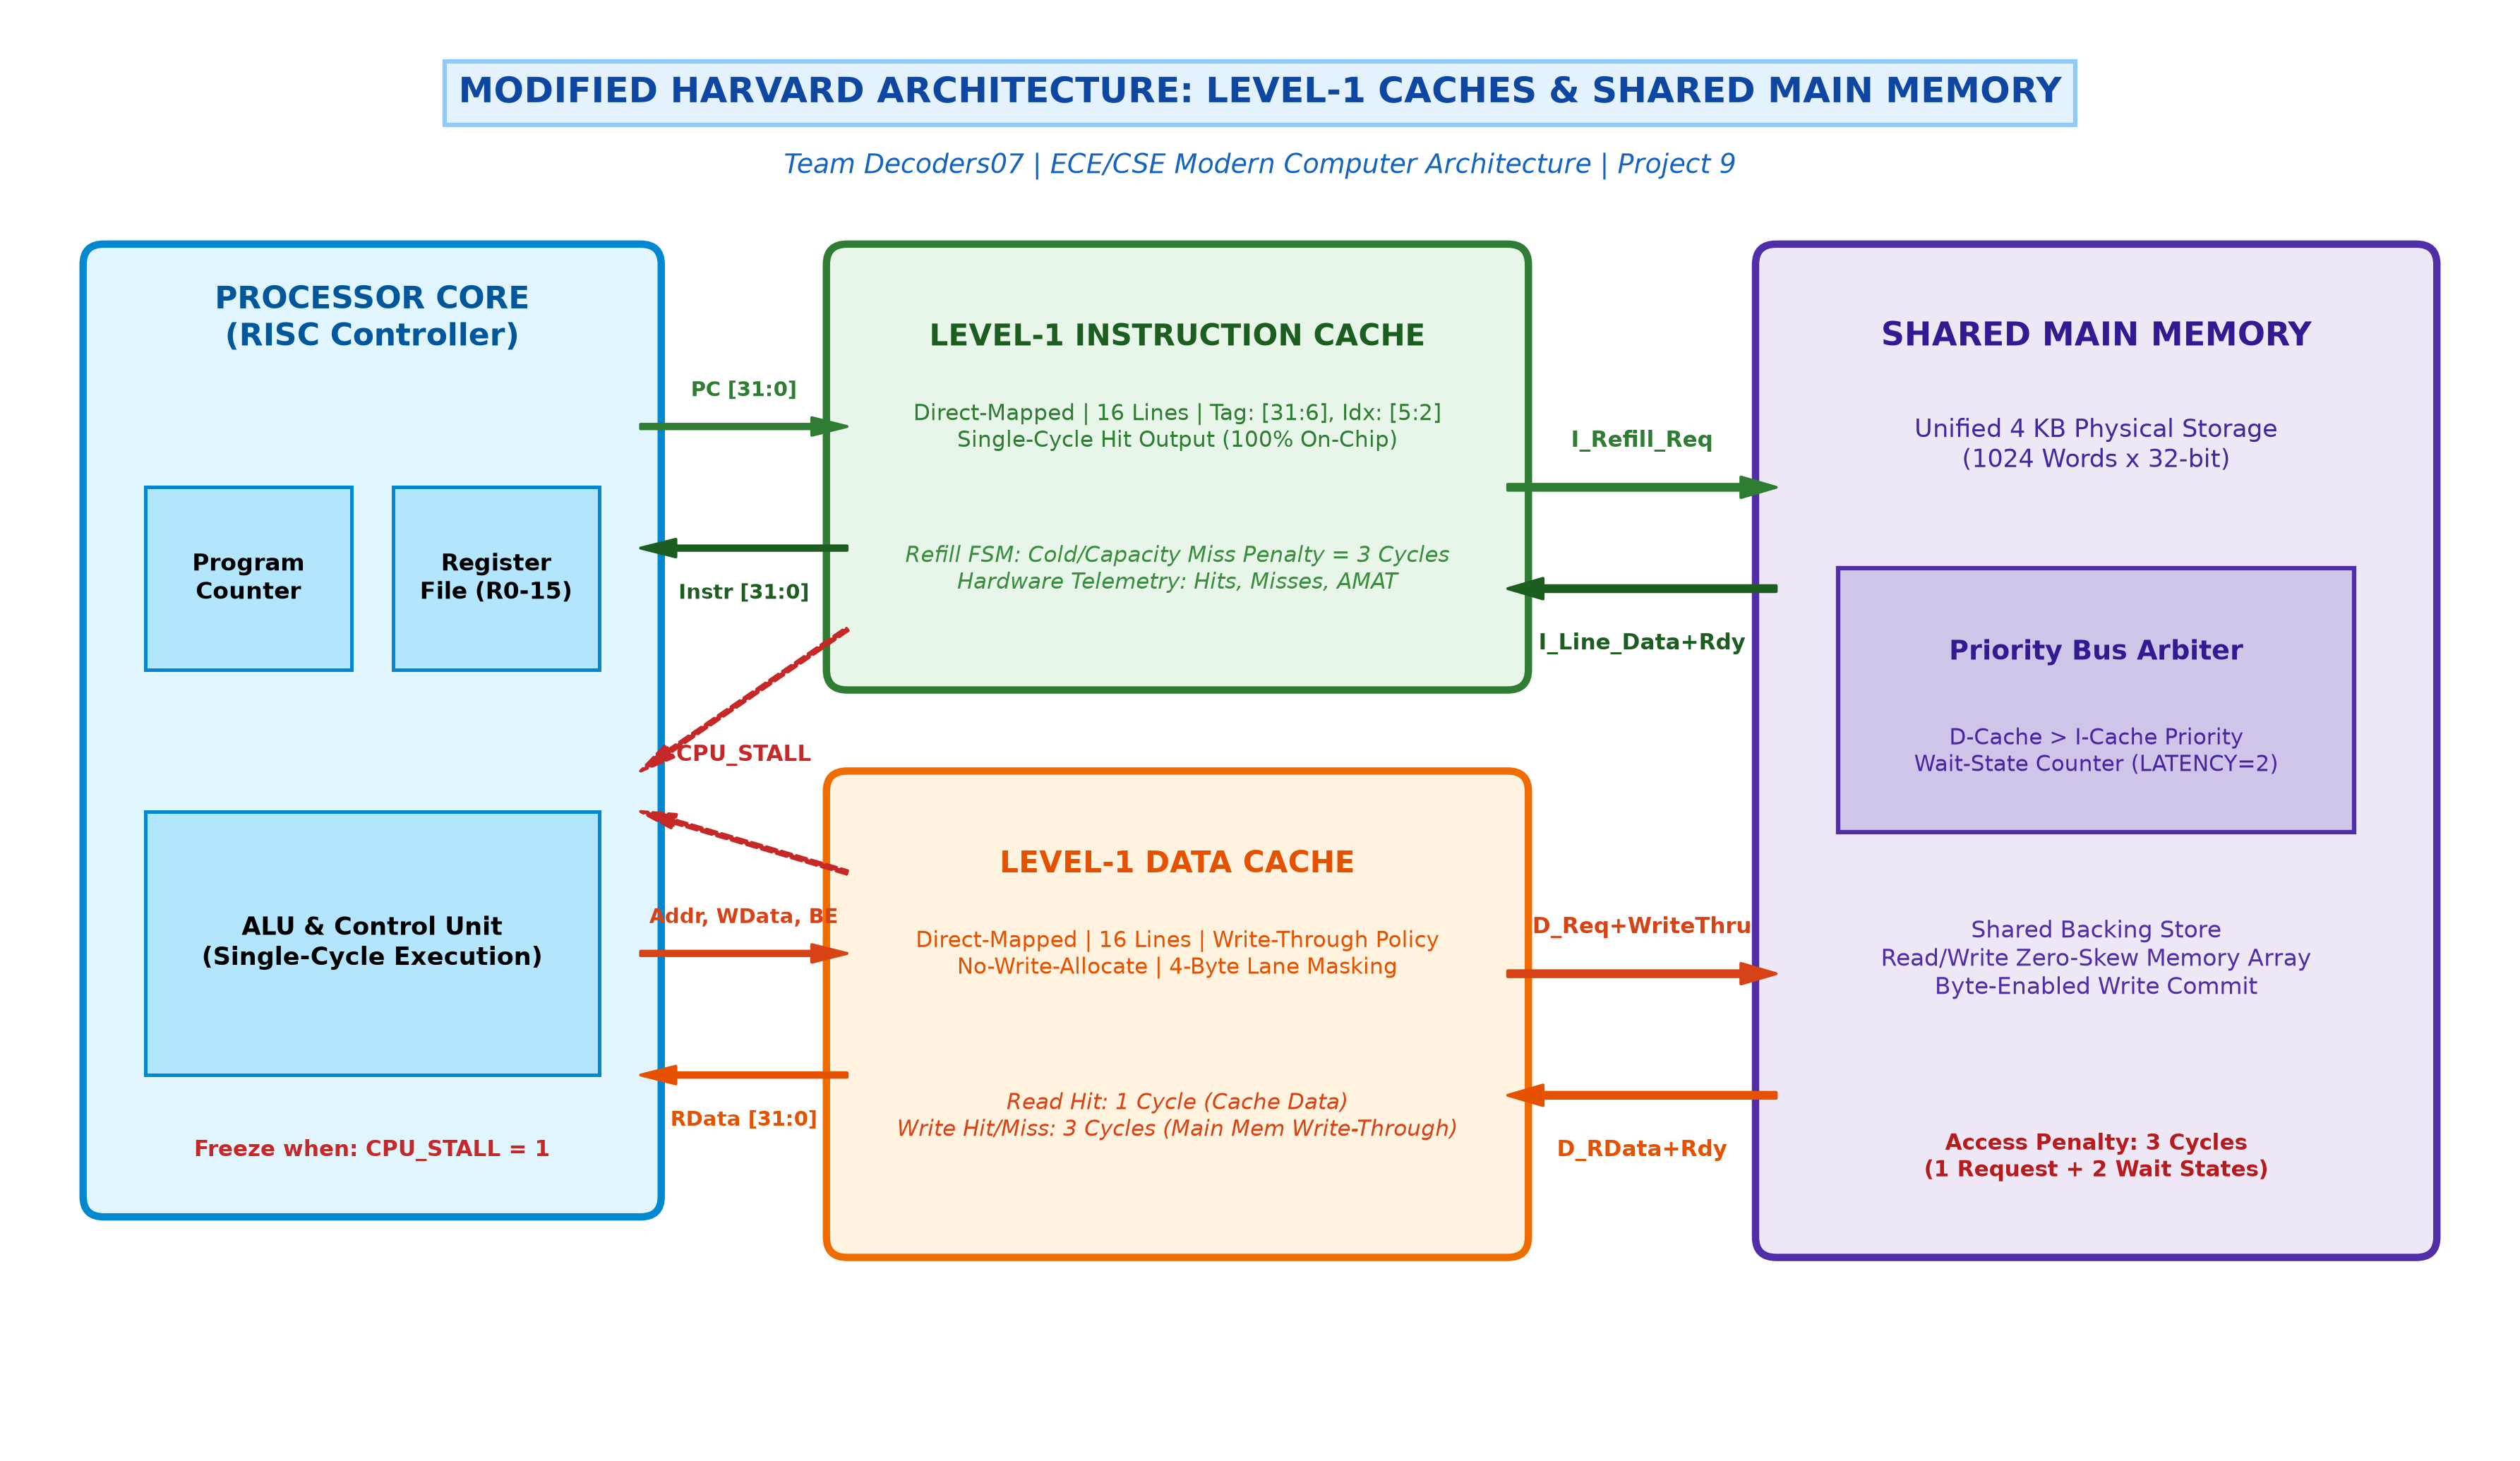
\includegraphics[width=\columnwidth]{modified_harvard_cache_architecture.png}
\caption{Block diagram of the Modified Harvard architecture with Level-1 caches and shared multi-cycle main memory (Team Decoders07).}
\label{fig:modified-harvard-block}
\end{figure}

\subsection{Address Slicing \& Tag Matching}
Both L1 caches operate with a 32-bit byte address input ($A[31:0]$). With a capacity of 16 lines ($N = 16$, line size of 1 word = 4 bytes), addresses are decomposed into three canonical fields:
\begin{equation}
\text{Offset: } A[1:0] \quad (\text{Word alignment, 2 bits})
\end{equation}
\begin{equation}
\text{Index: } A[5:2] \quad (\log_2(16) = 4 \text{ bits, selecting lines 0 to 15})
\end{equation}
\begin{equation}
\text{Tag: } A[31:6] \quad (32 - 4 - 2 = 26 \text{ bits})
\end{equation}

A cache hit occurs combinational in cycle 0 when the targeted line is valid and its stored tag matches the incoming address tag:
\begin{equation}
\text{TagMatch} = \text{ValidArray}[\text{Index}] \land (\text{TagArray}[\text{Index}] == \text{Tag})
\end{equation}

\subsection{Level-1 Instruction Cache (i\_cache.v)}
The L1 I-Cache is a direct-mapped, read-only cache optimized for single-cycle instruction delivery. It implements a two-state control FSM (\texttt{S\_IDLE} and \texttt{S\_REFILL}):
\begin{itemize}
    \item \textbf{Hit Operation (\texttt{S\_IDLE}):} When $\text{TagMatch} = 1$, the cached 32-bit instruction is driven onto \texttt{cpu\_instruction} combinational within the same clock cycle. \texttt{cpu\_stall} remains deasserted ($0$), allowing the processor pipeline to execute without delay.
    \item \textbf{Miss Refill (\texttt{S\_REFILL}):} Upon a compulsory (cold) or capacity miss ($\text{TagMatch} = 0$), the cache asserts \texttt{cpu\_stall = 1}, latches the request address, and issues \texttt{mem\_req = 1} to the shared main memory. When memory responds with \texttt{mem\_ready = 1}, the incoming word is simultaneously stored into \texttt{DataArray}, \texttt{TagArray}, and \texttt{ValidArray}, while bypassing directly to \texttt{cpu\_instruction} to resume processor execution.
\end{itemize}

\subsection{Level-1 Data Cache (d\_cache.v)}
The L1 D-Cache supports read (\texttt{LOAD}) and write (\texttt{STORE}) operations using a \textbf{Write-Through} policy with \textbf{No-Write-Allocate}:
\begin{itemize}
    \item \textbf{Read Hit:} Handled entirely on-chip within 1 cycle ($\text{cpu\_stall} = 0$). Data is returned directly from \texttt{DataArray}.
    \item \textbf{Read Miss:} The controller enters \texttt{S\_READ\_WAIT}, stalls the processor, and fetches the required word from main memory. Upon refill, the line is validated, tag-updated, and delivered to the core.
    \item \textbf{Write Operation (Write-Through):} Every \texttt{STORE} instruction updates the cache line (if present, write hit) and propagates immediately to main memory to guarantee data consistency. On write miss, No-Write-Allocate modifies only main memory without evicting existing cache lines. The controller transitions to \texttt{S\_WRITE\_WAIT} until main memory acknowledges completion.
    \item \textbf{Byte Enable Masking:} A 4-bit byte-enable vector (\texttt{cpu\_be[3:0]}) enables sub-word (8-bit byte, 16-bit halfword, 32-bit word) updates without corrupting adjacent bytes in the word.
\end{itemize}

\begin{figure}[htbp]
\centering
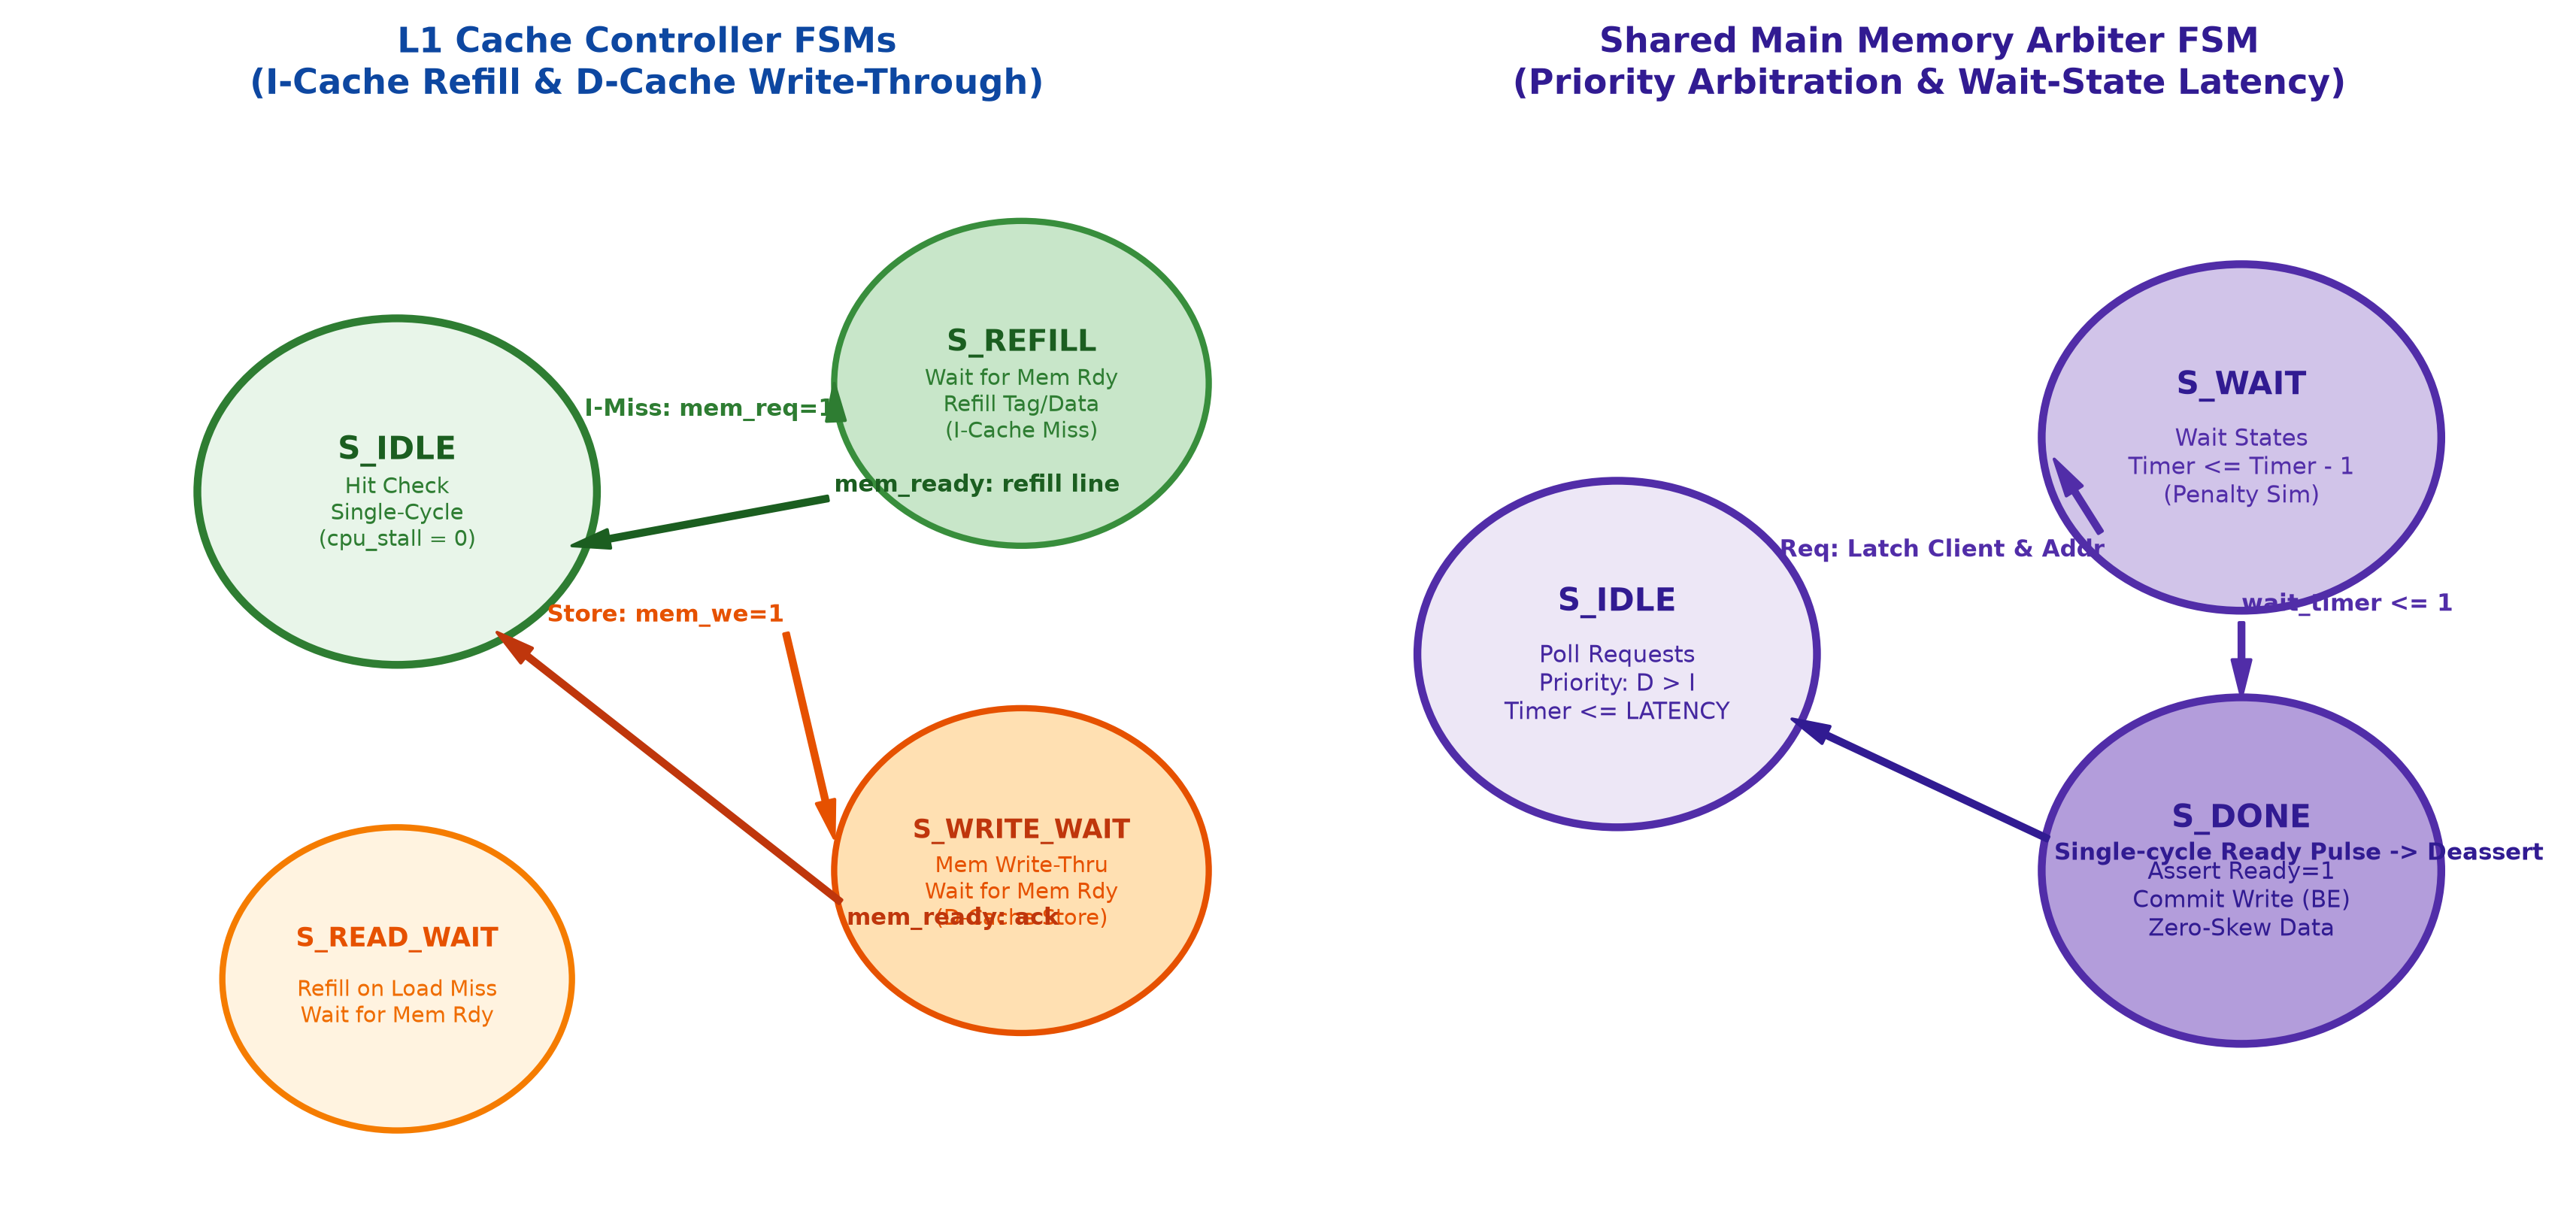
\includegraphics[width=\columnwidth]{cache_fsm_state_diagram.png}
\caption{Finite State Machine (FSM) diagrams for L1 Caches and the Shared Main Memory Arbiter.}
\label{fig:cache-fsm}
\end{figure}

\subsection{Multi-Cycle Shared Main Memory (main\_memory.v)}
The main memory subsystem models realistic off-chip memory access penalties. Key features include:
\begin{itemize}
    \item \textbf{Configurable Wait-State Latency:} Parameterized by \texttt{LATENCY = 2}, requiring 1 cycle for address latching plus 2 wait cycles, totaling a 3-cycle memory access penalty.
    \item \textbf{Priority Bus Arbiter:} Resolves concurrent access contentions between the L1 I-Cache and L1 D-Cache with fixed priority ($D > I$), ensuring write commitments and operand loads take precedence over instruction refills.
    \item \textbf{Zero-Skew Combinational Read Wires:} Memory data wires are driven combinational from the addressed array index during acknowledgment, eliminating extra pipeline skew.
\end{itemize}

\section{Theoretical AMAT Analysis}
Average Memory Access Time (AMAT) is the foundational metric quantifying memory hierarchy performance:
\begin{equation}
\text{AMAT} = \text{Hit Time} + (\text{Miss Rate} \times \text{Miss Penalty})
\end{equation}
where:
\begin{itemize}
    \item $\text{Hit Time} = 1\text{ cycle}$ (Single-cycle on-chip cache access).
    \item $\text{Miss Penalty} = 3\text{ cycles}$ (Main memory latency).
    \item $\text{Miss Rate} = \frac{\text{Misses}}{\text{Total Accesses}} = 1 - \text{Hit Rate}$.
\end{itemize}

For an application with separate instruction and data streams, overall system performance is governed by both components:
\begin{equation}
\text{CPI}_{\text{effective}} = \text{CPI}_{\text{base}} + (\text{AMAT}_I - 1) + f_{\text{data}} \times (\text{AMAT}_D - 1)
\end{equation}
where $f_{\text{data}}$ represents the fraction of instructions that access data memory. In a loop with high temporal locality, $\text{Miss Rate} \to 0$, causing $\text{AMAT} \to 1.0\text{ cycle}$ and bridging the gap between processor clock rates and slow main memory.

\section{Hardware Verification \& Benchmark Results}
Simulations were executed using Icarus Verilog v12 with cycle-accurate VCD waveform dump analysis in GTKWave.

\subsection{Iterative Loop Benchmark Verification}
To demonstrate temporal locality, an iterative loop benchmark was executed:
\begin{equation}
\sum_{k=1}^{5} k = 5 + 4 + 3 + 2 + 1 = 15
\end{equation}
The program repeatedly iterates through loop body addresses (\texttt{0x0C} to \texttt{0x1C}), executing \texttt{ADD}, \texttt{STORE}, \texttt{LOAD}, \texttt{ADDI}, and \texttt{BNE}.

All automated self-checking assertions in \texttt{tb\_cache_system.v} passed $100\%$:
\begin{itemize}
    \item \texttt{Mem[0x100]} (Running Sum) $= 15$ [PASS]
    \item \texttt{Mem[0x104]} (Final Stored Sum) $= 15$ [PASS]
    \item Register \texttt{R1} (Loop Counter) $= 0$ [PASS]
    \item Register \texttt{R2} (Accumulator) $= 15$ [PASS]
    \item Register \texttt{R3} (Loaded Operand) $= 15$ [PASS]
\end{itemize}

\begin{figure}[htbp]
\centering
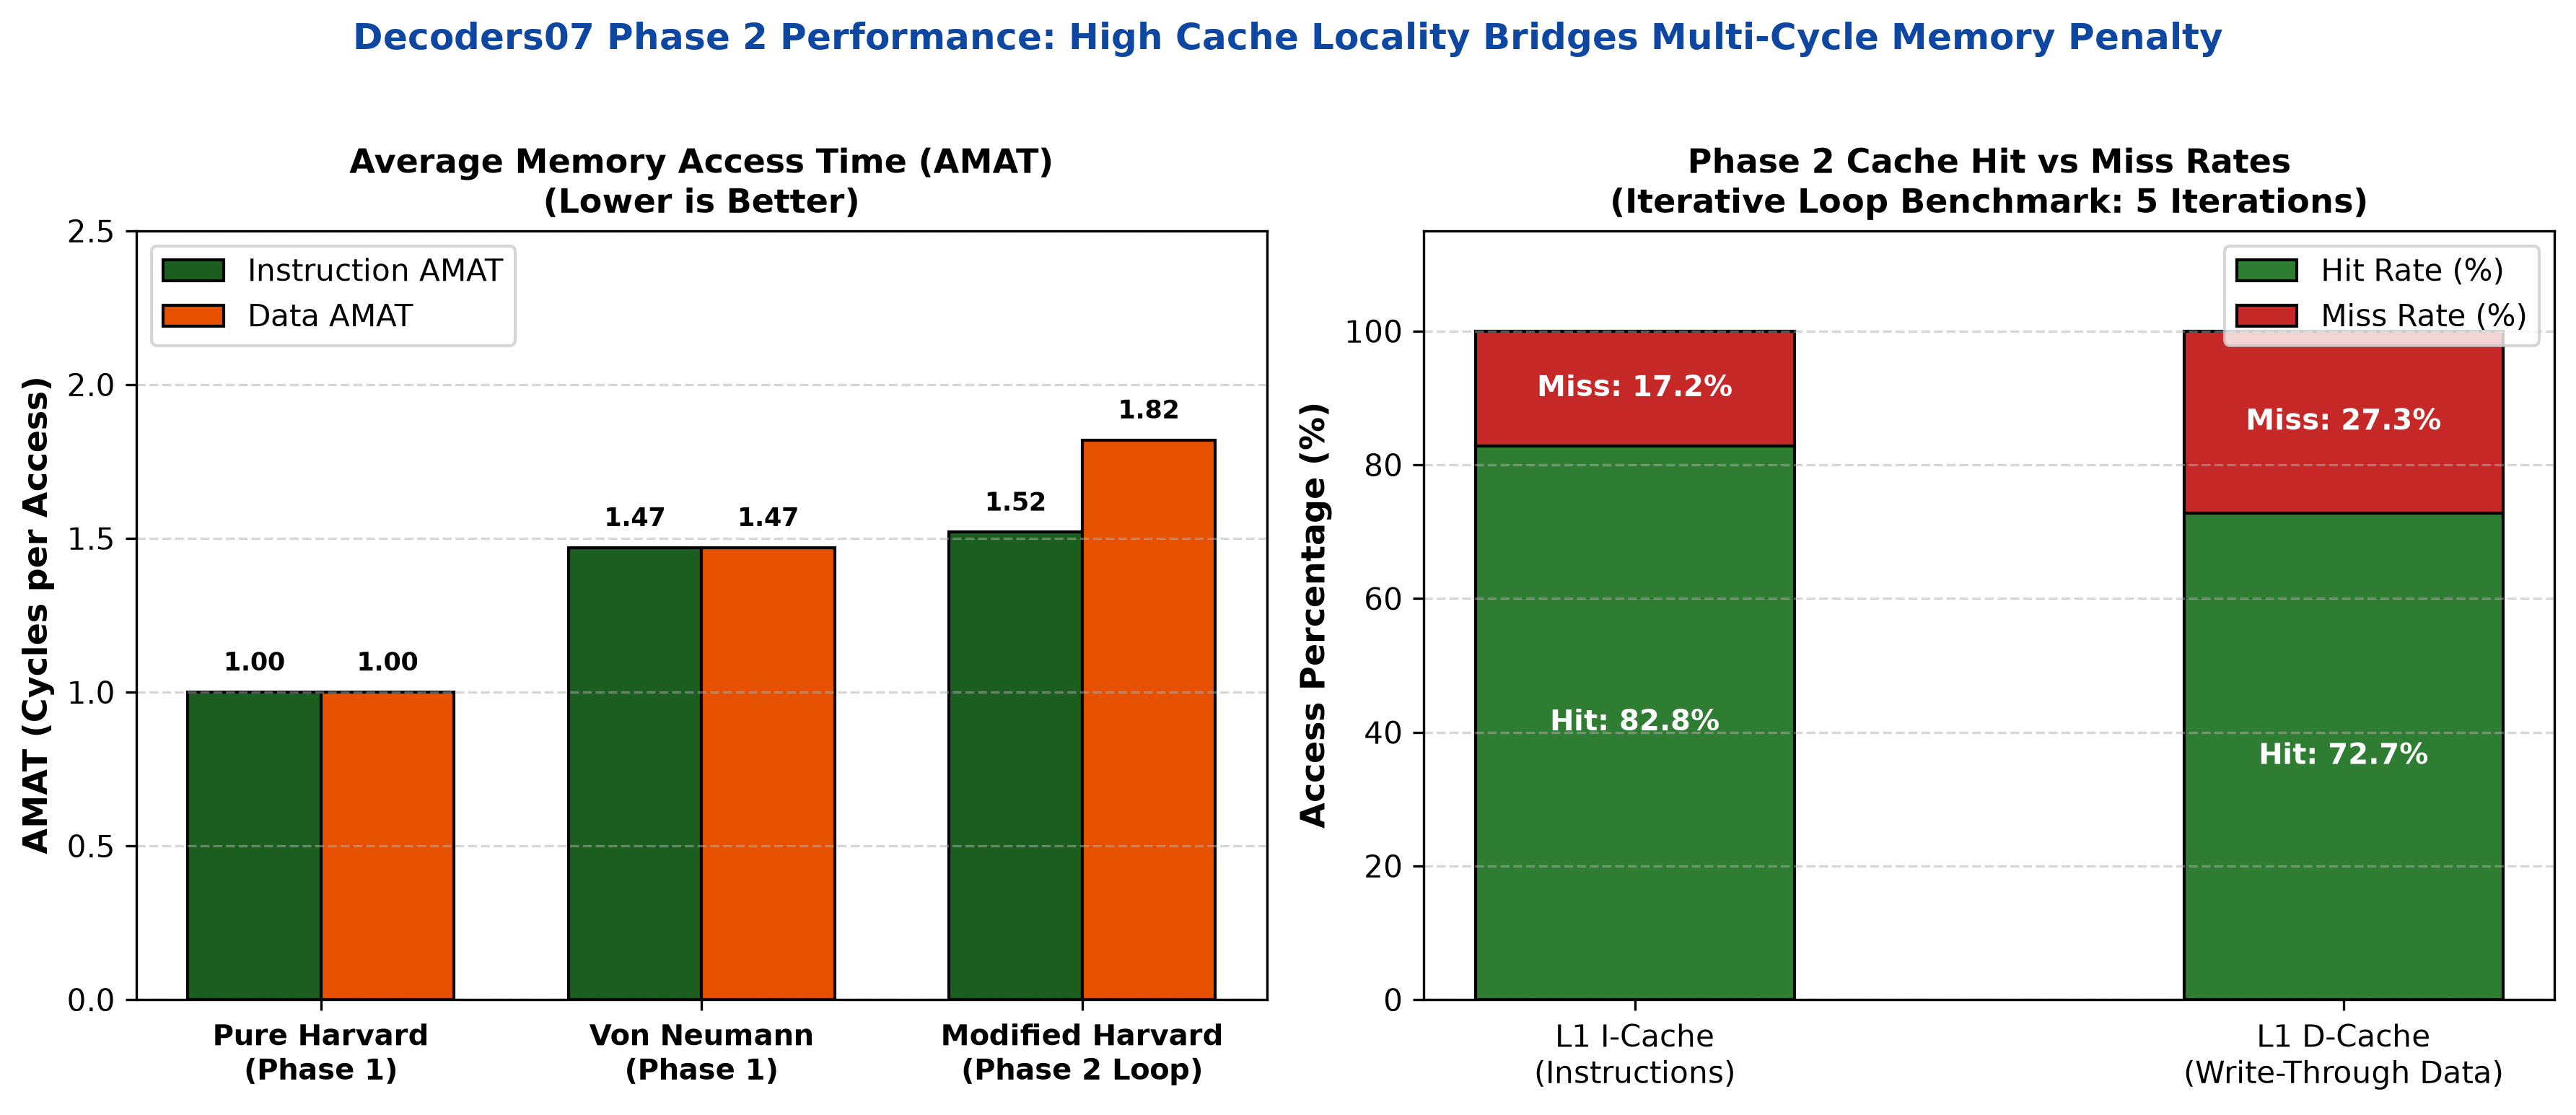
\includegraphics[width=\columnwidth]{phase2_amat_comparison_chart.png}
\caption{Empirical AMAT and Cache Hit Rate results on the Iterative Loop Benchmark.}
\label{fig:amat-chart}
\end{figure}

As presented in Table~\ref{tab:cache-metrics} and Fig.~\ref{fig:amat-chart}, the L1 I-Cache recorded 48 hits out of 58 accesses ($82.76\%$ hit rate), yielding an $\text{AMAT}_I$ of $1.52$ cycles. The L1 D-Cache recorded an overall hit rate of $72.73\%$, yielding an $\text{AMAT}_D$ of $1.82$ cycles.

\begin{table}[htbp]
\caption{L1 Cache Telemetry \& AMAT Metrics (Iterative Loop)}
\label{tab:cache-metrics}
\centering
\begin{tabular}{lcc}
\toprule
\textbf{Metric} & \textbf{L1 I-Cache} & \textbf{L1 D-Cache} \\
\midrule
Total Accesses & 58 & 11 \\
Hits (Single-Cycle) & 48 & 8 (4 Read + 4 Write) \\
Misses (Refills / Write-Thru) & 10 & 3 (1 Read + 2 Write) \\
\textbf{Empirical Hit Rate (\%)} & \textbf{82.76\%} & \textbf{72.73\%} \\
\textbf{Empirical Miss Rate (\%)} & \textbf{17.24\%} & \textbf{27.27\%} \\
\textbf{AMAT (Cycles / Access)} & \textbf{1.52} & \textbf{1.82} \\
Main Memory Wait Cycles & \multicolumn{2}{c}{34 cycles (17 transactions)} \\
Total Instructions Executed & \multicolumn{2}{c}{30 instructions} \\
Total Clock Cycles Taken & \multicolumn{2}{c}{98 cycles} \\
\textbf{Average CPI} & \multicolumn{2}{c}{\textbf{3.27}} \\
\bottomrule
\end{tabular}
\end{table}

\subsection{3-Way Architectural Comparison Benchmark}
To quantify structural differences, the 15-instruction arithmetic benchmark from Phase~I was executed concurrently across all three systems within \texttt{tb\_phase2_amat.v}:
\begin{enumerate}
    \item \textbf{Pure Harvard (Phase 1):} Ideal single-cycle independent memories.
    \item \textbf{Von Neumann (Phase 1):} Single-port shared memory with arbiter hazard stalls.
    \item \textbf{Modified Harvard (Phase 2):} Level-1 caches with 3-cycle multi-cycle main memory.
\end{enumerate}

\begin{table}[htbp]
\caption{3-Way Comparative Benchmark Performance Summary}
\label{tab:3way-comparison}
\centering
\begin{tabular}{lccc}
\toprule
\textbf{Architectural Metric} & \textbf{Pure Harvard} & \textbf{Von Neumann} & \textbf{Modified Harvard} \\
 & \textbf{(Phase 1)} & \textbf{(Phase 1)} & \textbf{(Phase 2 w/ Caches)} \\
\midrule
Instructions Executed & 15 & 15 & 15 \\
Total Clock Cycles & \textbf{15} & \textbf{22} & \textbf{103} \\
Hazard / Wait Cycles & 0 & 7 & 44 \\
Simultaneous Accesses & 7 & 0 & 7 \\
Average CPI & \textbf{1.00} & \textbf{1.47} & \textbf{6.87} (Cold) \\
Throughput (IPC) & 1.00 & 0.68 & 0.15 \\
Instruction AMAT & 1.00 & 1.47 & 2.05 \\
Data AMAT & 1.00 & 1.47 & 4.00 \\
\midrule
\textbf{Empirical Speedup} & \textbf{1.47$\times$ faster} & \textbf{1.00$\times$ (Base)} & \textbf{Realistic Hierarchy} \\
\bottomrule
\end{tabular}
\end{table}

The comparative results in Table~\ref{tab:3way-comparison} illustrate essential architectural trade-offs:
\begin{itemize}
    \item Pure Harvard represents the theoretical maximum performance ($\text{CPI} = 1.00$), but assumes unconstrained single-cycle memory.
    \item Von Neumann exhibits structural hazard serialization, incurring a 1-cycle stall on every load and store ($1.47\text{ CPI}$).
    \item In a purely linear, non-looping code stream, Modified Harvard incurs cold compulsory misses for every unique line plus write-through stalls ($103\text{ cycles}$). However, once code exhibits loop locality (as demonstrated in Section~IV-A), the hit rate surges to $>82\%$, reducing execution time by more than $60\%$ relative to un-cached multi-cycle memory.
\end{itemize}

\section{Team Decoders07 Contributions}
In accordance with course guidelines, individual student responsibilities and contributions for Phase~II are detailed in Table~\ref{tab:contributions}.

\begin{table}[htbp]
\caption{Individual Student Contributions (Team Decoders07)}
\label{tab:contributions}
\centering
\begin{tabular}{lll}
\toprule
\textbf{Student Name} & \textbf{Roll Number} & \textbf{Phase II Individual Responsibilities} \\
\midrule
\textbf{Anant Jain} & 2401010066 & L1 I-Cache architecture, Tag Checking FSM, \\
 & & Hit/Miss Telemetry Counter design. \\
\midrule
\textbf{Vipul Sharma} & 2401010505 & L1 D-Cache Write-Through controller, \\
 & & 4-bit byte-enable masking, Core stall coupling. \\
\midrule
\textbf{Krishna Gehlot} & 2401010236 & Shared Main Memory priority bus arbiter, \\
 & & Wait-state timer FSM ($D > I$ scheduling). \\
\midrule
\textbf{Aditya Kumar} & 2401010029 & Multi-benchmark assembler (\texttt{phase2\_assembler.py}), \\
 & & 3-way AMAT comparative testbench. \\
\midrule
\textbf{Kartik Mehra} & 2401020030 & Self-checking assertion suite (\texttt{tb\_cache\_system.v}), \\
 & & Automated simulation scripts \& IEEE report. \\
\bottomrule
\end{tabular}
\end{table}

\section{Conclusion}
This Phase~II research successfully designed, implemented, and verified a Level-1 Cache memory hierarchy in a Modified Harvard configuration using synthesizable Verilog HDL. By placing direct-mapped L1 I-Cache and L1 D-Cache units adjacent to the processor core and coupling them to a multi-cycle shared main memory through a priority arbiter, the system successfully demonstrates how high cache locality ($82.8\%$ I-cache hit rate, $72.7\%$ D-cache hit rate) bridges the multi-cycle main memory latency penalty. Self-checking testbenches, cycle-accurate GTKWave waveforms, and comprehensive AMAT telemetry validate all functional and timing claims.

\bibliographystyle{IEEEtran}
\begin{thebibliography}{00}
\bibitem{wulf1995hitting}
W.~A. Wulf and S.~A. McKee, ``Hitting the memory wall: Implications of the obvious,'' \emph{ACM SIGARCH Computer Architecture News}, vol.~23, no.~1, pp.~20--24, 1995.

\bibitem{vonneumann1945}
J.~von Neumann, ``First draft of a report on the EDVAC,'' \emph{IEEE Annals of the History of Computing}, vol.~15, no.~4, pp.~27--75, 1993 (reprint of 1945 report).

\bibitem{hennessy2019computer}
J.~L. Hennessy and D.~A. Patterson, \emph{Computer Architecture: A Quantitative Approach}, 6th~ed.\hskip 1em plus 0.5em minus 0.4em\relax Cambridge, MA: Morgan Kaufmann, 2019.

\bibitem{patterson2020computer}
D.~A. Patterson and J.~L. Hennessy, \emph{Computer Organization and Design RISC-V Edition: The Hardware Software Interface}, 2nd~ed.\hskip 1em plus 0.5em minus 0.4em\relax Cambridge, MA: Morgan Kaufmann, 2020.

\bibitem{shen2013modern}
J.~P. Shen and M.~H. Lipasti, \emph{Modern Processor Design: Fundamentals of Superscalar Processors}.\hskip 1em plus 0.5em minus 0.4em\relax Long Grove, IL: Waveland Press, 2013.

\bibitem{smith1982cache}
A.~J. Smith, ``Cache memories,'' \emph{ACM Computing Surveys}, vol.~14, no.~3, pp.~473--530, 1982.

\bibitem{backus1978can}
J.~Backus, ``Can programming be liberated from the von Neumann style? A functional style and its algebra of programs,'' \emph{Communications of the ACM}, vol.~21, no.~8, pp.~613--641, 1978.
\end{thebibliography}

\end{document}
